\documentclass[12pt,a4paper]{article}

% ─── Page Layout ───────────────────────────────────────────────────────────────
\usepackage[a4paper, margin=0.8in, headheight=14pt]{geometry}

% ─── Fonts (XeLaTeX) ───────────────────────────────────────────────────────────
\usepackage{fontspec}
\usepackage{unicode-math}
\setmainfont{TeX Gyre Pagella}
\setmonofont[Scale=0.88]{TeX Gyre Cursor}
\setmathfont{Latin Modern Math}

% ─── Packages ──────────────────────────────────────────────────────────────────
\usepackage{xcolor}
\usepackage{colortbl}
\usepackage{titlesec}
\usepackage{enumitem}
\usepackage{tabularx}
\usepackage{booktabs}
\usepackage{array}
\usepackage{amsmath}
\usepackage{tikz}
\usetikzlibrary{shapes.geometric, arrows.meta, positioning, calc, fit, decorations.pathreplacing}
\usepackage{tcolorbox}
\tcbuselibrary{skins, breakable}
\usepackage{hyperref}
\usepackage{fancyhdr}
\usepackage{graphicx}
\usepackage{microtype}
\hyphenpenalty=10000
\exhyphenpenalty=10000
\sloppy
\usepackage{caption}
\usepackage{setspace}
\usepackage{multirow}
\usepackage{tocloft}

% ─── Q&A helper ────────────────────────────────────────────────────────────────
\newcommand{\Q}[1]{\textbf{#1}\par\noindent\ignorespaces}

% ─── Colour Palette ────────────────────────────────────────────────────────────
\definecolor{myred}{RGB}{196,30,58}
\definecolor{mydark}{RGB}{30,30,50}
\definecolor{mygreen}{RGB}{14,120,80}
\definecolor{myteal}{RGB}{0,130,140}
\definecolor{myamber}{RGB}{180,100,0}
\definecolor{mypurple}{RGB}{100,30,160}
\definecolor{mygray}{RGB}{246,247,249}
\definecolor{mgframe}{RGB}{180,185,200}
\definecolor{watermark}{RGB}{145,150,170}
\definecolor{hdrred}{RGB}{250,232,235}
\definecolor{hdrgreen}{RGB}{220,244,233}
\definecolor{hdrteal}{RGB}{220,242,244}
\definecolor{hdramber}{RGB}{253,242,215}
\definecolor{hdrpurple}{RGB}{238,228,255}
\definecolor{hdrgray}{RGB}{238,240,245}
\definecolor{rowalt}{RGB}{250,251,253}

% ─── Section Formatting ────────────────────────────────────────────────────────
\titleformat{\section}
  {\large\bfseries\color{myred}}{\thesection.}{0.5em}{}
  [\vspace{1pt}{\color{myred}\rule{\linewidth}{0.8pt}}]
\titleformat{\subsection}
  {\normalsize\bfseries\color{myteal}}{\thesubsection}{0.5em}{}
\titlespacing*{\section}{0pt}{18pt}{7pt}
\titlespacing*{\subsection}{0pt}{11pt}{4pt}

% ─── Paragraph ─────────────────────────────────────────────────────────────────
\setlength{\parindent}{0pt}
\setlength{\parskip}{4pt}

% ─── TOC Styling ───────────────────────────────────────────────────────────────
\renewcommand{\cfttoctitlefont}{\large\bfseries\color{myred}}
\renewcommand{\cftaftertoctitle}{\par\noindent{\color{myred}\rule{\linewidth}{0.8pt}}}
\setlength{\cftbeforetoctitleskip}{0pt}
\setlength{\cftaftertoctitleskip}{6pt}
\renewcommand{\cftsecfont}{\normalsize\bfseries\color{mydark}}
\renewcommand{\cftsecpagefont}{\normalsize\bfseries\color{mydark}}
\renewcommand{\cftsecleader}{\cftdotfill{\cftdotsep}}
\setlength{\cftbeforesecskip}{7pt}
\renewcommand{\cftsubsecfont}{\small\color{mydark}}
\renewcommand{\cftsubsecpagefont}{\small\color{mydark}}
\setlength{\cftbeforesubsecskip}{3pt}
\setlength{\cftsubsecindent}{1.4em}

% ─── Table helpers ─────────────────────────────────────────────────────────────
\renewcommand{\arraystretch}{1.45}
\setlength{\tabcolsep}{6pt}
\arrayrulecolor{mydark}
\newcolumntype{B}[1]{>{\small\bfseries\raggedright\arraybackslash}m{#1}}
\newcolumntype{Y}{>{\small\raggedright\arraybackslash}X}
\renewcommand{\tabularxcolumn}[1]{m{#1}}

% ─── Header / Footer ───────────────────────────────────────────────────────────
\pagestyle{fancy}
\fancyhf{}
\fancyhead[L]{\small\color{myred}\textbf{OE-EC704B}\;\color{mydark}--- Optimization Technique}
\fancyhead[R]{\small\color{myteal}\textbf{Module 5 Notes}}
\fancyfoot[C]{\small\color{mydark}\thepage}
\fancyfoot[R]{\small\color{watermark}\textit{\copyright\ Biraj}}
\renewcommand{\headrulewidth}{0.5pt}
\renewcommand{\footrulewidth}{0.3pt}

% ─── Hyperref ──────────────────────────────────────────────────────────────────
\hypersetup{
  colorlinks=true, linkcolor=myteal, urlcolor=myteal,
  pdfauthor={Biraj Sarkar},
  pdftitle={OE-EC704B --- Module 5 Notes}
}

% ─── tcolorbox styles ──────────────────────────────────────────────────────────
\tcbset{
  tikzbox/.style={
    colback=mygray, colframe=mgframe, boxrule=0.6pt, arc=4pt,
    left=8pt, right=8pt, top=6pt, bottom=6pt,
    colbacktitle=mgframe, coltitle=mydark,
    fonttitle=\small\bfseries
  },
  defbox/.style={
    colback=hdrgreen, colframe=mygreen, boxrule=0.8pt, arc=4pt,
    left=9pt, right=9pt, top=6pt, bottom=6pt,
    colbacktitle=mygreen, coltitle=white,
    fonttitle=\small\bfseries
  },
  formulabox/.style={
    colback=hdrteal, colframe=myteal, boxrule=0.8pt, arc=4pt,
    left=9pt, right=9pt, top=7pt, bottom=7pt,
    colbacktitle=myteal, coltitle=white,
    fonttitle=\small\bfseries
  },
  examplebox/.style={
    colback=hdramber, colframe=myamber, boxrule=0.8pt, arc=4pt,
    left=9pt, right=9pt, top=6pt, bottom=6pt,
    colbacktitle=myamber, coltitle=white,
    fonttitle=\small\bfseries
  },
  masonbox/.style={
    colback=hdrpurple, colframe=mypurple, boxrule=0.8pt, arc=4pt,
    left=9pt, right=9pt, top=6pt, bottom=6pt,
    colbacktitle=mypurple, coltitle=white,
    fonttitle=\small\bfseries
  },
  exambox/.style={
    colback=hdrpurple, colframe=mypurple, boxrule=1pt, arc=5pt,
    left=10pt, right=10pt, top=8pt, bottom=8pt,
    colbacktitle=mypurple, coltitle=white,
    fonttitle=\bfseries,
    breakable, title after break={\textbf{Frequently Asked / Viva Questions (contd.)}}}
}
\tcbset{breakable}

% ─── TikZ styles ───────────────────────────────────────────────────────────────
\tikzset{
  block/.style={rectangle, draw=myteal, fill=hdrteal,
    text width=2.4cm, align=center, minimum height=0.95cm,
    font=\small, rounded corners=3pt, line width=0.7pt},
  redblock/.style={rectangle, draw=myred, fill=hdrred,
    text width=2.4cm, align=center, minimum height=0.95cm,
    font=\small, rounded corners=3pt, line width=0.7pt},
  netnode/.style={rectangle, draw=myteal, fill=hdrteal,
    text width=1.5cm, align=center, minimum height=0.8cm,
    font=\small, rounded corners=3pt, line width=0.7pt},
  sumjunc/.style={circle, draw=myamber, fill=hdramber,
    minimum size=0.62cm, font=\small, line width=0.8pt},
  snode/.style={circle, draw=mypurple, fill=hdrpurple,
    minimum size=0.55cm, font=\footnotesize, line width=0.7pt},
  arrow/.style={-Stealth, thick, color=mydark},
  redarrow/.style={-Stealth, thick, color=myred},
  line/.style={thick, color=mydark}
}

% ═══════════════════════════════════════════════════════════════════════════════
\begin{document}
% ═══════════════════════════════════════════════════════════════════════════════

\begin{center}
  {\LARGE\bfseries\color{myred} OE-EC704B --- Optimization Technique}\\[5pt]
  {\normalsize\color{mydark} Semester VII \quad$\bullet$\quad 3L:0T:0P \quad$\bullet$\quad 3 Credits}\\[3pt]
  {\normalsize\color{myteal}\textbf{Module 5 Exam Notes: Constrained Optimization Algorithms}}\\[3pt]
  {\small\color{mydark} CGEC \;$|$\; B.Tech ECE (2023--27) \;$|$\; \textit{Biraj Sarkar}}
\end{center}
\vspace{2pt}
\noindent{\color{myred}\rule{\linewidth}{1.5pt}}
\vspace{2pt}

\hypersetup{linkcolor=mydark}
\tableofcontents
\hypersetup{linkcolor=myteal}
\newpage

% ===============================================================================
\section{Characteristics of Constrained Problems}
% ===============================================================================

Constrained optimization restricts the search space to a feasible region. Let us analyze the constraint boundaries:

\begin{tcolorbox}[defbox, title={Active vs. Inactive Constraints}]
At a candidate design point $\mathbf{x}$:
\begin{itemize}[leftmargin=*, itemsep=2.5pt, topsep=0pt]
  \item An inequality constraint $g_j(\mathbf{x}) \le 0$ is said to be \textbf{Active} if $g_j(\mathbf{x}) = 0$. The point lies exactly on the boundary of that constraint.
  \item It is \textbf{Inactive} if $g_j(\mathbf{x}) < 0$. The constraint is satisfied, and the point lies in the interior of the feasible space.
  \item It is \textbf{Violated} if $g_j(\mathbf{x}) > 0$. The design point is infeasible.
\end{itemize}
All equality constraints $h_k(\mathbf{x}) = 0$ must be active at all feasible points.
\end{tcolorbox}

\begin{tcolorbox}[tikzbox, title={Feasible Region and Constrained Optimum}]
\centering
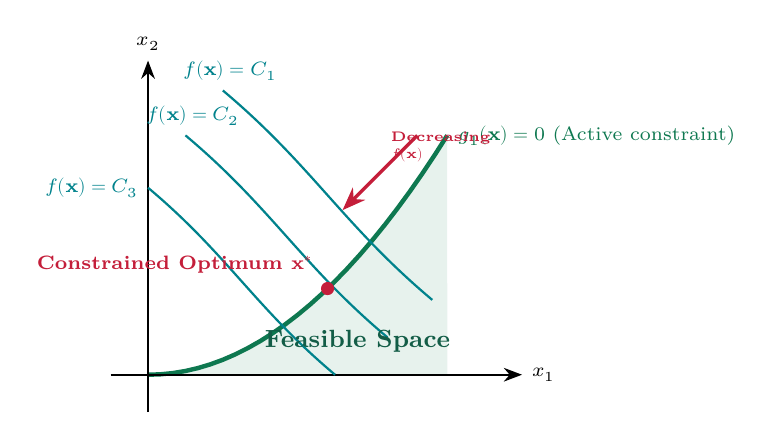
\begin{tikzpicture}[scale=0.95]
  % Feasible area shading
  \fill[mygreen!10] (0,0) plot[domain=0:4] (\x, {0.2*\x*\x}) -- (4,0) -- cycle;
  \draw[ultra thick, color=mygreen] (0,0) plot[domain=0:4] (\x, {0.2*\x*\x}) node[right, font=\scriptsize] {$g_1(\mathbf{x}) = 0$ (Active constraint)};
  
  % Axes
  \draw[-Stealth, thick] (-0.5,0) -- (5,0) node[right, font=\scriptsize\bfseries] {$x_1$};
  \draw[-Stealth, thick] (0,-0.5) -- (0,4.2) node[above, font=\scriptsize\bfseries] {$x_2$};
  
  % Contours of f(x)
  \draw[thick, color=myteal] (1.0, 3.8) to[out=-40, in=140] (3.8, 1.0);
  \node[above, font=\scriptsize, color=myteal] at (1.1,3.8) {$f(\mathbf{x}) = C_1$};
  
  \draw[thick, color=myteal] (0.5, 3.2) to[out=-40, in=140] (3.2, 0.5);
  \node[above, font=\scriptsize, color=myteal] at (0.6,3.2) {$f(\mathbf{x}) = C_2$};
  
  \draw[thick, color=myteal] (0.0, 2.5) to[out=-40, in=140] (2.5, 0.0);
  \node[left, font=\scriptsize, color=myteal] at (0.0,2.5) {$f(\mathbf{x}) = C_3$};
  
  % Decreasing Direction Arrow
  \draw[-Stealth, very thick, color=myred] (3.6, 3.2) -- (2.6, 2.2) 
    node[midway, above right, font=\tiny\bfseries\color{myred}, align=left] {Decreasing\\$f(\mathbf{x})$};

  % Feasible text
  \node[color=mygreen!70!mydark, font=\small\bfseries] at (2.8, 0.45) {Feasible Space};
  
  % Optimum Point
  \coordinate (opt) at (2.4, 1.152);
  \fill[myred] (opt) circle (2.5pt);
  \node[above left, font=\scriptsize\bfseries, color=myred, xshift=-2pt, yshift=2pt] at (opt) {Constrained Optimum $\mathbf{x}^*$};
\end{tikzpicture}
\end{tcolorbox}

% ===============================================================================
\section{Direct Constrained Optimization Methods}
% ===============================================================================

Direct methods evaluate only function values and directly handle constraints by adjusting candidate coordinates.

\subsection{Box's Complex Method}
Box's Complex Method is an extension of the Nelder-Mead Simplex method designed to handle inequality constraints:
\begin{itemize}[leftmargin=*, itemsep=2.5pt]
  \item Uses a geometric shape called a \textbf{Complex} consisting of $k \ge n+1$ vertices (typically $k = 2n$).
  \item If a generated reflection point violates an inequality constraint, it is moved halfway toward the centroid of the remaining feasible points until it becomes feasible.
\end{itemize}

\subsection{Kelly's Cutting Plane Method}
Kelly's Cutting Plane Method solves non-linear convex constrained problems:
\begin{enumerate}[label=\textbf{\arabic*.}, leftmargin=*, itemsep=2.5pt]
  \item Linearizes all non-linear constraints using first-order Taylor expansions to form a linear programming (LP) relaxation.
  \item Solves the LP relaxation. If the solution is infeasible for the original non-linear constraints, it adds a new linear inequality constraint (a \textbf{Cutting Plane}) that slices off the infeasible LP solution.
  \item Repeats the process until convergence, generating a sequence of tightening linear hulls.
\end{enumerate}

% ===============================================================================
\section{Indirect Methods (Transformation Techniques)}
% ===============================================================================

Transformation techniques reformulate a constrained problem into an equivalent sequence of unconstrained problems.

\subsection{Exterior Penalty Function Method}
The exterior penalty method starts search in the infeasible region and penalizes constraint violations, forcing iterations toward the feasible boundary.

\begin{tcolorbox}[formulabox, title={Exterior Penalty Function Formulation}]
The unconstrained penalty objective function $\Phi$ is defined as:
\begin{equation}
  \Phi(\mathbf{x}, r_p) = f(\mathbf{x}) + r_p \sum_{j=1}^m \left[ \max\left(0, g_j(\mathbf{x})\right) \right]^2 + \frac{1}{r_p} \sum_{k=1}^p \left[ h_k(\mathbf{x}) \right]^2
\end{equation}
Where $r_p$ is a positive penalty parameter.
\par\vspace{3pt}
*Algorithm:*
\begin{enumerate}[label=\textbf{\arabic*.}, leftmargin=*, itemsep=2.5pt]
  \item Select an initial penalty value $r_p^{(1)}$ (usually small) and minimize $\Phi(\mathbf{x}, r_p^{(1)})$ unconstrained.
  \item Increase the parameter: $r_p^{(k+1)} = c \cdot r_p^{(k)}$ (where $c > 1$).
  \item Re-minimize $\Phi$. As $r_p \to \infty$, the sequence of unconstrained minima converges to the constrained optimum $\mathbf{x}^*$.
\end{enumerate}
\end{tcolorbox}

\subsection{Interior Penalty (Barrier) Function Method}
The interior penalty method starts inside the feasible region and creates a barrier at the boundary that prevents iterations from escaping into the infeasible space.

\begin{tcolorbox}[formulabox, title={Interior Barrier Function Formulations}]
The unconstrained barrier objective function $\Phi$ is defined using one of two barriers:
\begin{itemize}[leftmargin=*, itemsep=3pt, topsep=0pt]
  \item \textbf{Inverse Barrier Function:}
    \begin{equation}
      \Phi(\mathbf{x}, r_k) = f(\mathbf{x}) - r_k \sum_{j=1}^m \frac{1}{g_j(\mathbf{x})}
    \end{equation}
  \item \textbf{Logarithmic Barrier Function:}
    \begin{equation}
      \Phi(\mathbf{x}, r_k) = f(\mathbf{x}) - r_k \sum_{j=1}^m \ln\left[ -g_j(\mathbf{x}) \right]
    \end{equation}
\end{itemize}
Where $r_k$ is the positive barrier parameter.
\par\vspace{3pt}
*Algorithm:*
\begin{enumerate}[label=\textbf{\arabic*.}, leftmargin=*, itemsep=2.5pt]
  \item Start at a strictly feasible point. Minimize $\Phi(\mathbf{x}, r_k^{(1)})$.
  \item Decrease the parameter: $r_k^{(k+1)} = d \cdot r_k^{(k)}$ (where $0 < d < 1$).
  \item Re-minimize. As $r_k \to 0$, the barrier effect weakens at the boundary, allowing convergence to the boundary optimum $\mathbf{x}^*$.
\end{enumerate}
\end{tcolorbox}

% ===============================================================================
\section{Convex Optimization Methods}
% ===============================================================================

Convex optimization is a special class of optimization with unique mathematical guarantees.

\begin{tcolorbox}[defbox, title={Convex Programming Problem}]
A constrained optimization problem is a \textbf{Convex Programming Problem} if:
\begin{enumerate}[label=\textbf{\arabic*.}, leftmargin=*, itemsep=2pt, topsep=0pt]
  \item The objective function $f(\mathbf{x})$ is convex.
  \item All inequality constraints $g_j(\mathbf{x}) \le 0$ are convex functions.
  \item All equality constraints $h_k(\mathbf{x}) = 0$ are linear (affine) functions.
\end{enumerate}
\end{tcolorbox}

\textbf{Theorem:} For a convex programming problem, \textbf{any local minimum is guaranteed to be the global minimum}, eliminating the risk of getting trapped in local sub-optimal states.

\newpage

% ===============================================================================
% MANDATORY QUICK REVISION PAGE
% ===============================================================================
\begin{center}
  {\large\bfseries\color{myred} Quick Revision --- Module 5}\\[3pt]
  {\small\color{mydark} Constrained Optimization $|$ OE-EC704B}
\end{center}
\noindent{\color{myred}\rule{\linewidth}{1.2pt}}
\vspace{4pt}

\begin{tcolorbox}[formulabox, title={\textbf{Key Concepts \& Formulations}}]
\renewcommand{\arraystretch}{1.45}
\begin{tabularx}{\linewidth}{B{5.0cm} X}
Active Inequality & $g_j(\mathbf{x}^*) = 0$ \quad (optimum lies on the constraint boundary). \\[4pt]
Inactive Inequality & $g_j(\mathbf{x}^*) < 0$ \quad (constraint is satisfied with slack). \\[4pt]
Exterior Penalty $\Phi$ & $\Phi = f(\mathbf{x}) + r_p \sum [\max(0, g_j)]^2$ \quad (where $r_p \to \infty$). \\[4pt]
Inverse Interior Barrier & $\Phi = f(\mathbf{x}) - r_k \sum \frac{1}{g_j}$ \quad (where $r_k \to 0$). \\[4pt]
Logarithmic Barrier & $\Phi = f(\mathbf{x}) - r_k \sum \ln(-g_j)$ \quad (where $r_k \to 0$). \\[4pt]
Convex Definition & $f(\lambda \mathbf{x} + (1-\lambda)\mathbf{y}) \le \lambda f(\mathbf{x}) + (1-\lambda)f(\mathbf{y})$ for $\lambda \in [0, 1]$. \\
\end{tabularx}
\end{tcolorbox}

\begin{tcolorbox}[defbox, title={\textbf{One-Line Definitions}}]
\begin{itemize}[leftmargin=*, itemsep=2.5pt, topsep=0pt]
  \item \textbf{Active Constraint:} A constraint whose boundary passes directly through the current design point.
  \item \textbf{Complex Method:} A constrained direct search method utilizing $2n$ vertices to explore bounded spaces.
  \item \textbf{Transformation Technique:} Reformulating constrained problems into sequential unconstrained formulations.
  \item \textbf{Exterior Penalty Method:} A transformation technique that approaches the boundary from the infeasible design region.
  \item \textbf{Interior Barrier Method:} A transformation technique that approaches the boundary from strictly within the feasible region.
  \item \textbf{Convex Function:} A function where a line segment connecting any two points on its graph lies above or on the graph.
\end{itemize}
\end{tcolorbox}

\begin{tcolorbox}[exambox, title={\textbf{Frequently Asked / Viva Questions}}]
\begin{enumerate}[topsep=0pt, label=\textbf{Q\arabic*.}, itemsep=5pt]
  \item \Q{What is the difference between active and inactive constraints at an optimum point?}
    An active constraint satisfies $g_j(\mathbf{x}^*) = 0$ (lies on the boundary). An inactive constraint satisfies $g_j(\mathbf{x}^*) < 0$ (lies inside the boundary) and does not limit the local optimum.
  \item \Q{Compare the search paths of the Exterior Penalty and Interior Barrier methods.}
    The exterior penalty method starts from an infeasible point and moves inward toward the feasible boundary as $r_p \to \infty$. The interior barrier method starts from a strictly feasible point and moves outward toward the boundary as $r_k \to 0$.
  \item \Q{Why does the Interior Barrier method require a strictly feasible starting point?}
    Because the barrier terms (such as $1/g_j$ or $\ln(-g_j)$) are mathematically undefined or return complex/imaginary values in the infeasible region ($g_j(\mathbf{x}) > 0$).
  \item \Q{State Sylvester's conditions for a function to be strictly convex.}
    A function is strictly convex if its Hessian matrix $H(\mathbf{x})$ is positive definite (all eigenvalues $> 0$) at all points in the design space.
  \item \Q{What is the main advantage of Convex Programming?}
    Any local minimum of a convex programming problem is guaranteed to be the global minimum.
  \item \Q{Explain the concept behind Kelly's Cutting Plane method.}
    It linearizes the non-linear constraints to solve an approximating linear program. It then iteratively adds linear constraint inequalities (cutting planes) to cut off infeasible areas.
  \item \Q{Why are equality constraints challenging for the Interior Barrier method?}
    Because equality constraints $h_k(\mathbf{x}) = 0$ define a region with zero thickness, leaving no "interior" space to start a strictly feasible search path.
  \item \Q{How does Box's Complex method handle constraint violations?}
    If a generated point is infeasible, it is iteratively retracted halfway toward the centroid of the remaining feasible points until it becomes feasible.
  \item \Q{Write down the logarithmic barrier objective function expression.}
    $\Phi(\mathbf{x}, r_k) = f(\mathbf{x}) - r_k \sum_{j=1}^m \ln(-g_j(\mathbf{x}))$.
  \item \Q{What is the physical meaning of the penalty parameter $r_p$ in the exterior penalty method?}
    It acts as a scaling coefficient for constraint violations. As $r_p \to \infty$, the penalty for violating constraints becomes extremely large, forcing the unconstrained optimizer to find a feasible solution.
\end{enumerate}
\end{tcolorbox}

\end{document}
